\documentclass[12pt]{report}
\usepackage[utf8]{inputenc}
\usepackage[T2A]{fontenc}
\usepackage[russian]{babel}

\usepackage{amsmath,amsfonts,amssymb,amsthm,mathtools}
\DeclarePairedDelimiter\abs{\lvert}{\rvert}

\usepackage{pgfplots}
\usepackage{filecontents}
\usepackage{indentfirst}
\usepackage{eucal}
\usepackage{enumitem}
% Для \abs{}
\usepackage{commath}
\usepackage{float}
\frenchspacing

% Для нормальных переносов
\sloppy

\usetikzlibrary{datavisualization}
\usetikzlibrary{datavisualization.formats.functions}

\usepackage[left=2cm,right=2cm, top=2cm,bottom=2cm,bindingoffset=0cm]{geometry}
% Для измененных титулов глав:
\usepackage{titlesec, blindtext, color} % подключаем нужные пакеты
\definecolor{gray75}{gray}{0.75} % определяем цвет
\newcommand{\hsp}{\hspace{20pt}} % длина линии в 20pt
% titleformat определяет стиль
\titleformat{\chapter}[hang]{\Huge\bfseries}{\thechapter\hsp\textcolor{gray75}{|}\hsp}{0pt}{\Huge\bfseries}

% plot
\usepackage{xcolor}
\usepackage{stmaryrd}
\usepackage{wasysym}
\usetikzlibrary{datavisualization}
\usetikzlibrary{datavisualization.formats.functions}

% листинги
\usepackage{listings}
\usepackage{graphicx}
\usepackage{caption}
\usepackage{textcomp}
\lstset{
    language = C,
    basicstyle=\small\sffamily,
    numbers=left,
    numberstyle=\tiny,
    stepnumber=1,
    numbersep=5pt,
    showspaces=false,
    showstringspaces=false,
    showtabs=false,
    frame=single,
    tabsize=2,
    captionpos=t,
    breaklines=true,
    breakatwhitespace=false,
    escapeinside={\#*}{*)},
    literate=	{а}{{\selectfont\char224}}1
			    {б}{{\selectfont\char225}}1
			    {в}{{\selectfont\char226}}1
			    {г}{{\selectfont\char227}}1
			    {д}{{\selectfont\char228}}1
			    {е}{{\selectfont\char229}}1
			    {ё}{{\"e}}1
			    {ж}{{\selectfont\char230}}1
			    {з}{{\selectfont\char231}}1
			    {и}{{\selectfont\char232}}1
			    {й}{{\selectfont\char233}}1
			    {к}{{\selectfont\char234}}1
			    {л}{{\selectfont\char235}}1
			    {м}{{\selectfont\char236}}1
			    {н}{{\selectfont\char237}}1
			    {о}{{\selectfont\char238}}1
			    {п}{{\selectfont\char239}}1
			    {р}{{\selectfont\char240}}1
			    {с}{{\selectfont\char241}}1
			    {т}{{\selectfont\char242}}1
			    {у}{{\selectfont\char243}}1
			    {ф}{{\selectfont\char244}}1
			    {х}{{\selectfont\char245}}1
			    {ц}{{\selectfont\char246}}1
			    {ч}{{\selectfont\char247}}1
			    {ш}{{\selectfont\char248}}1
			    {щ}{{\selectfont\char249}}1
			    {ъ}{{\selectfont\char250}}1
			    {ы}{{\selectfont\char251}}1
			    {ь}{{\selectfont\char252}}1
			    {э}{{\selectfont\char253}}1
			    {ю}{{\selectfont\char254}}1
			    {я}{{\selectfont\char255}}1
			    {А}{{\selectfont\char192}}1
			    {Б}{{\selectfont\char193}}1
			    {В}{{\selectfont\char194}}1
			    {Г}{{\selectfont\char195}}1
			    {Д}{{\selectfont\char196}}1
			    {Е}{{\selectfont\char197}}1
			    {Ё}{{\"E}}1
			    {Ж}{{\selectfont\char198}}1
			    {З}{{\selectfont\char199}}1
			    {И}{{\selectfont\char200}}1
			    {Й}{{\selectfont\char201}}1
			    {К}{{\selectfont\char202}}1
			    {Л}{{\selectfont\char203}}1
			    {М}{{\selectfont\char204}}1
			    {Н}{{\selectfont\char205}}1
			    {О}{{\selectfont\char206}}1
			    {П}{{\selectfont\char207}}1
			    {Р}{{\selectfont\char208}}1
			    {С}{{\selectfont\char209}}1
			    {Т}{{\selectfont\char210}}1
			    {У}{{\selectfont\char211}}1
			    {Ф}{{\selectfont\char212}}1
			    {Х}{{\selectfont\char213}}1
			    {Ц}{{\selectfont\char214}}1
			    {Ч}{{\selectfont\char215}}1
			    {Ш}{{\selectfont\char216}}1
			    {Щ}{{\selectfont\char217}}1
			    {Ъ}{{\selectfont\char218}}1
			    {Ы}{{\selectfont\char219}}1
			    {Ь}{{\selectfont\char220}}1
			    {Э}{{\selectfont\char221}}1
			    {Ю}{{\selectfont\char222}}1
			    {Я}{{\selectfont\char223}}1
}
\captionsetup[lstlisting]{justification=raggedright, singlelinecheck=off}

\begin{document}
%\def\chaptername{} % убирает "Глава"
    % Титульник
\thispagestyle{empty}
\begin{titlepage}
	\noindent \begin{minipage}{0.15\textwidth}
				  
\includegraphics[width=\linewidth]{img/b_logo}
	\end{minipage}
	\noindent\begin{minipage}{0.9\textwidth}
				 \centering
				 \textbf{Министерство науки и высшего образования Российской Федерации}\\
				 \textbf{Федеральное государственное бюджетное образовательное учреждение высшего образования}\\
				 \textbf{~~~«Московский государственный технический университет имени Н.Э.~Баумана}\\
				 \textbf{(национальный исследовательский университет)»}\\
				 \textbf{(МГТУ им. Н.Э.~Баумана)}
	\end{minipage}

	\noindent\rule{18cm}{3pt}
	\newline\newline
	\noindent ФАКУЛЬТЕТ $\underline{\text{«Информатика и системы управления»}}$ \newline\newline
	\noindent КАФЕДРА $\underline{\text{«Программное обеспечение ЭВМ и информационные технологии»}}$\newline\newline\newline\newline\newline


	\begin{center}
		\noindent\begin{minipage}{1.3\textwidth}
					 \centering
					 \Large\textbf{  Отчет по лабораторной работе №4}\newline
					 \textbf{по дисциплине "Операционные системы"}\newline\newline
		\end{minipage}
	\end{center}

	\noindent\textbf{Тема} $\underline{\text{Процессы. Системные вызовы fork() и exec()}}$\newline\newline
	\noindent\textbf{Студент} $\underline{\text{Шацкий Р.Е.}}$\newline\newline
	\noindent\textbf{Группа} $\underline{\text{ИУ7-55Б}}$\newline\newline
	\noindent\textbf{Оценка (баллы)} $\underline{\text{~~~~~~~~~~~~~~~~~~~~~~~~~~~}}$\newline\newline
	\noindent\textbf{Преподаватели} $\underline{\text{Рязанова Н.Ю.}}$\newline\newline\newline

	\begin{center}
		\vfill
		Москва~---~\the\year
		~г.
	\end{center}
\end{titlepage}

    
    \section*{Задание 1. Процессы-сироты.}
    В программе создаются не менее двух потомков.
    В потомках вызывается sleep().
    Чтобы предок гарантированно завершился раньше своих потомков.
    Продемонстрировать с помощью соответствующего вывода информацию об идентификаторах процессов и их группе.
    Продемонстрировать «усыновление».
    Для этого надо в потомках вывести идентификаторы:
    собственный, предка, группы до блокировки и после блокировки.
    
    \begin{lstlisting}[label=code:fork, caption=Процессы-сироты, language=C]
    	#include <stdio.h>
    	#include <stdlib.h>
    	
    	enum error_t {
    		no_error,
    		fork_failure
    	};
    	
    	#define PROC_COUNT 3
    	#define SLEEP_TIME 1
    	
    	int main() {
    		int children[PROC_COUNT];
    		printf("\n Предок --- PID: %d, GROUP: %d\n", getpid(), getpgrp());
    		
    		for (int i = 0; i < PROC_COUNT; ++i) {
    			int child_pid = fork();
    			
    			if (child_pid == -1) {
    				perror("Ошибка fork\n");
    				return fork_failure;
    			}
    			else if (child_pid == 0) {
    				printf("Для потомка до усыновления No%d --- PID: %d, PPID: %d, GROUP: %d\n", i + 1, getpid(), getppid(), getpgrp());
    				sleep(SLEEP_TIME * 4);
    				printf("Для потомка после усыновления No%d --- PID: %d, PPID: %d, GROUP: %d\n", i + 1, getpid(), getppid(), getpgrp());
    				return no_error;
    			}
    			else {
    				sleep(SLEEP_TIME);
    				children[i] = child_pid;
    			}
    		}
    		
    		printf("Процессы, созданные предком:\n");
    		for (int i = 0; i < PROC_COUNT; ++i) {
    			printf("Потомок No%d --- PID: %d, ", i + 1, children[i]);
    		}
    		printf("\b\b\nПредок завершился\n");
    		
    		return no_error;
    	}
    \end{lstlisting}

	\begin{figure}[H]
		
		\centering
		
		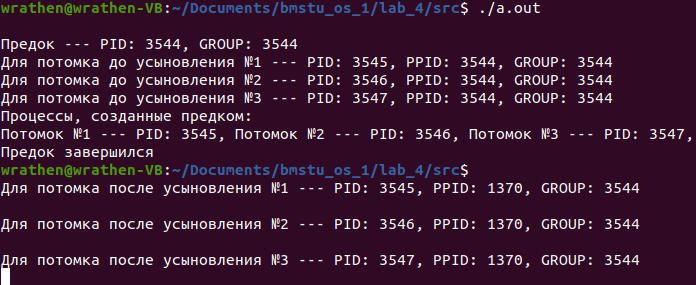
\includegraphics[width=\linewidth]{img/task_01.png}
		\caption{Демонстрация работы программы (задание №1).}
		
		\label{fig:task_01}
		
	\end{figure}

	\section*{Задание 2.}
	Предок ждет завершения своих потомком, используя системный вызов wait().
	Вывод соответствующих сообщений на экран.
	В программе необходимо, чтобы предок выполнял анализ кодов завершения потомков.
	
	\begin{lstlisting}[label=code:wait, caption=wait(), language=C]
		#include <stdio.h>
		#include <stdlib.h>
		#include <wait.h>
		
		enum error_t {
			no_error,
			fork_failure
		};
		
		#define PROC_COUNT 3
		#define SLEEP_TIME 1
		
		int main() {
			int children[PROC_COUNT];
			printf("\nПредок --- PID: %d, GROUP: %d\n", getpid(), getpgrp());
			
			for (int i = 0; i < PROC_COUNT; ++i) {
				int child_pid = fork();
				
				if (child_pid == -1) {
					perror("Can't fork");
					return fork_failure;
				}
				else if (child_pid == 0) {
					sleep(SLEEP_TIME);
					printf("Для потомка No%d --- PID: %d, PPID: %d, GROUP: %d\n", i + 1, getpid(), getppid(), getpgrp());
					return 0;
				}
				else {
					children[i] = child_pid;
				}
			}
			
			printf("Процессы, созданные предком:\n");
			for (int i = 0; i < PROC_COUNT; ++i) {
				int status;
				int stat_value = 0;
				
				pid_t child_pid = wait(&status);
				printf("Потомок с PID = %d завершился. Статус: %d\n", children[i], status);
				
				if (WIFEXITED(stat_value)) {
					printf("\tПотомок завершился нормально. Код завершения: %d\n", WEXITSTATUS(stat_value));
				}
				else if (WIFSIGNALED(stat_value)) {
					printf("\tПотомок завершился неперехватываемым сигналом. Номер сигнала: %d\n", WTERMSIG(stat_value));
				}
				else if (WIFSTOPPED(stat_value)) {
					printf("\tПотомок остановился. Номер сигнала: %d\n", WSTOPSIG(stat_value));
				}
			}
			printf("Предок завершился\n");
			
			return no_error;
		}
	\end{lstlisting}

	\begin{figure}[H]
	
		\centering
		
		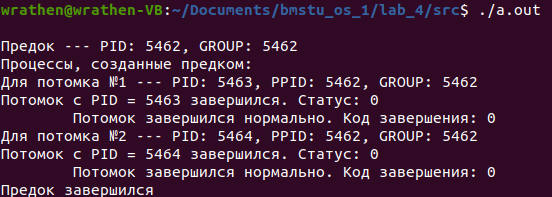
\includegraphics[width=\linewidth]{img/task_02.png}
		\caption{Демонстрация работы программы (задание №2).}
		
		\label{fig:task_02}
	
	\end{figure}

	\section*{Задание 3.}
	Потомки переходят на выполнение других программ, которые передаются
	системному вызову exec() в качестве параметра.
	Потомки должны выполнять разные программы.
	Предок ждет завершения своих потомков с анализом кодов завершения.
	На экран выводятся соответствующие сообщения.
	
	С помощью вызова exec() выполняются программы из первых лабораторных работ
	на курсе по языку C: 
	
	Определить нормальный вес человека и индекс массы его тела по формулам:
	{h * t / 240} и {m / h\^2}, 
	где h - рост человека (измеряемый в сантиметрах в первой формуле и в метрах - во второй);
	t - длина окружности грудной клетки (в сантиметрах); m - вес (в килограммах). 
	Порядок ввода параметров: h, t, m (h в см, t в см, m в кг).
	
	\begin{lstlisting}[label=code:my_test, caption={Код программы weight\_index}, language=C]
		#include <stdio.h>
		
		int main(int argc, char* argv[])
		{
			for (int i = 0; i < argc; ++i) {
				printf("Аргумент No%d = %s\n", i, argv[i]);
			}
			
			float h, t, m;
			
			printf("Введите через пробел рост в см, длину окр. грудной клетки в см и вес в кг:\n");
			scanf("%f %f %f", &h, &t, &m);
			
			float weight = h * t / 240;
			float index = m / (h / 100) / (h / 100);
			
			printf("%.5f %.5f\n", weight, index);
			
			return 0;
		}
	\end{lstlisting}

	Треугольник задан координатами вершин. Определить тип треугольника.
	Ввод: x1, y1, x2, y2, x3, y3.
	Вывод: 0 - остроугольный, 1 - прямоугольный, 2 - тупоугольный.

	\begin{lstlisting}[label=code:my_test2, caption={Код программы triangle\_type}, language=C]
		#include <stdio.h>
		#include <math.h>
		
		int check(float a2, float b2, float c2)
		{
			float h = 1e-6;
			int result = 0;
			/* 90 degrees check */
			if (fabsf(a2 - b2 - c2) < h || fabsf(b2 - a2 - c2) < h || fabsf(c2 - b2 - a2) < h)
			{
				result = 1;
			}
			/* >90 degrees check */
			else if (b2 + c2 - a2 < 0 || b2 + a2 - c2 < 0 || a2 + c2 - b2 < 0)
			{
				result = 2;
			}
			return result;
		}
		
		int main(int argc, char* argv[])
		{
			for (int i = 0; i < argc; ++i) {
				printf("Аргумент No%d = %s\n", i, argv[i]);
			}
			
			printf("Введите координаты вершин треугольника:\n");
			float x1, y1, x2, y2, x3, y3;
			if (scanf("%f %f %f %f %f %f", &x1, &y1, &x2, &y2, &x3, &y3) != 6)
			{
				printf("Input error");
				return -1;
			}
			/* is it triangle check */
			if (fabsf((x1 - x3) * (y2 - y3) - (x2 - x3) * (y1 - y3)) < 1e-6)
			{
				printf("Input error");
				return -1;
			}
			
			float a2 = (x1 - x2) * (x1 - x2) + (y1 - y2) * (y1 - y2);
			float b2 = (x3 - x2) * (x3 - x2) + (y3 - y2) * (y3 - y2);
			float c2 = (x3 - x1) * (x3 - x1) + (y3 - y1) * (y3 - y1);
			
			printf("%d\n", check(a2, b2, c2));
			return 0;
		}
	\end{lstlisting}
	
	\begin{lstlisting}[label=code:exec, caption=exec(), language=C]
		#include <stdio.h>
		#include <stdlib.h>
		#include <wait.h>
		#include <string.h>
		
		enum error_t {
			no_error,
			fork_fail,
			exec_fail
		};
		
		#define PROC_COUNT 3
		#define SLEEP_TIME 2
		
		int main() {
			int children[PROC_COUNT];
			char *commands[PROC_COUNT] = {"./weight_index.out", "./triangle_type.out"};
			char *args[PROC_COUNT] = {"ПЕРВЫЙ", "__ВТОРОЙ__", ""};
			printf("Предок --- PID: %d, GROUP: %d\n", getpid(), getpgrp());
			
			for (int i = 0; i < PROC_COUNT; ++i) {
				int child_pid = fork();
				
				if (child_pid == -1) {
					perror("Ошибка fork'а");
					return fork_fail;
				}
				else if (child_pid == 0) {
					sleep(SLEEP_TIME);
					printf("Для потомка No%d --- PID: %d, PPID: %d, GROUP: %d\n", i + 1, getpid(), getppid(), getpgrp());
					
					int res = execlp(commands[i], args[i], 0);
					if (res == -1) {
						perror("Exec невозможен");
						return exec_fail;
					}
					
					return no_error;
				}
				else {
					children[i] = child_pid;
				}
			}
			
			printf("Процессы, созданные предком:\n");
			for (int i = 0; i < PROC_COUNT; ++i) {
				int status;
				int stat_value = 0;
				
				pid_t child_pid = wait(&status);
				printf("Потомок с PID = %d завершился. Статус: %d\n", children[i], status);
				
				if (WIFEXITED(stat_value)) {
					printf("\tПотомок завершился нормально. Код завершения: %d\n", WEXITSTATUS(stat_value));
				}
				else if (WIFSIGNALED(stat_value)) {
					printf("\tПотомок завершился неперехватываемым сигналом. Номер сигнала: %d\n", WTERMSIG(stat_value));
				}
				else if (WIFSTOPPED(stat_value)) {
					printf("\tПотомок остановился. Номер сигнала: %d\n", WSTOPSIG(stat_value));
				}
			}
			printf("Предок завершился\n");
			
			return no_error;
		}
	\end{lstlisting}

	\begin{figure}[H]
	
		\centering
		
		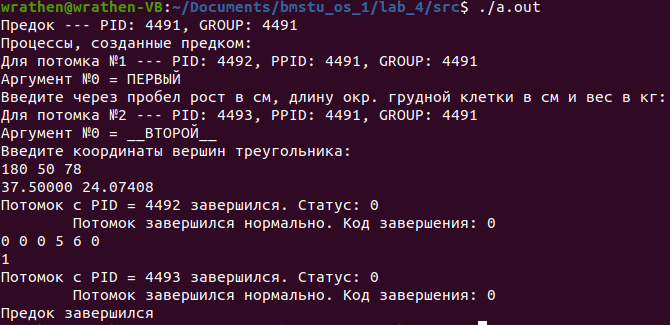
\includegraphics[width=\linewidth]{img/task_03.png}
		\caption{Демонстрация работы программы (задание №3).}
		
		\label{fig:task_03}
	
	\end{figure}

	\section*{Задание 4.}
	Предок и потомки обмениваются сообщениями через неименованный программный канал.
	Причем оба потомка пишут свои сообщения в один программный канал, а предок их считывает из канала.
	Потомки должны посылать предку разные сообщения по содержанию и размеру.
	Предок считывает сообщения от потомков и выводит их на экран.
	Предок ждет завершения своих потомков и анализирует код их завершения.
	Вывод соответствующих сообщений на экран.

	\begin{lstlisting}[label=code:pipe, caption=pipe(), language=C]
		#include <stdio.h>
		#include <stdlib.h>
		#include <wait.h>
		#include <string.h>
		
		enum error_t {
			no_error,
			fork_fail,
			exec_fail,
			pipe_fail
		};
		
		#define PROC_COUNT 3
		#define SLEEP_TIME 2
		#define STR_BUFF_SIZE 64
		
		int main() {
			int pipefd[2];  // [0] - чтение, [1] - запись
			if (pipe(pipefd) == -1) {
				perror("Ошибка pipe");
				return pipe_fail;
			}
			
			char *msgs[PROC_COUNT] = {"First msg\n", "Second msg\n", "Third message\n"};
			char str_buff[STR_BUFF_SIZE] = {0};
			
			int children[PROC_COUNT];
			printf("Предок --- PID: %d, GROUP: %d\n", getpid(), getpgrp());
			
			for (int i = 0; i < PROC_COUNT; ++i) {
				int child_pid = fork();
				
				if (child_pid == -1) {
					perror("Ошибка fork'а");
					return fork_fail;
				}
				else if (child_pid == 0) {
					printf("Для потомка No%d --- PID: %d, PPID: %d, GROUP: %d\n", i + 1, getpid(), getppid(), getpgrp());
					
					close(pipefd[0]);
					write(pipefd[1], msgs[i], strlen(msgs[i]));
					
					printf("Сообщение No%d отправлено потомку\n\n", i + 1);
					
					return no_error;
				}
				else {
					children[i] = child_pid;
				}
			}
			
			printf("Процессы, созданные предком:\n");
			for (int i = 0; i < PROC_COUNT; ++i) {
				int status;
				int stat_value = 0;
				
				pid_t child_pid = wait(&status);
				printf("Потомок с PID = %d завершился. Статус: %d\n", children[i], status);
				
				if (WIFEXITED(stat_value)) {
					printf("\tПотомок завершился нормально. Код завершения: %d\n\n", WEXITSTATUS(stat_value));
				}
				else if (WIFSIGNALED(stat_value)) {
					printf("\tПотомок завершился неперехватываемым сигналом. Номер сигнала: %d\n\n", WTERMSIG(stat_value));
				}
				else if (WIFSTOPPED(stat_value)) {
					printf("\tПотомок остановился. Номер сигнала: %d\n\n", WSTOPSIG(stat_value));
				}
			}
			
			close(pipefd[1]);
			read(pipefd[0], str_buff, STR_BUFF_SIZE);
			printf("Сообщения, полученные предком: %s", str_buff);
			
			printf("Предок завершился\n");
			return no_error;
		}
	\end{lstlisting}

	\begin{figure}[H]
		
		\centering
		
		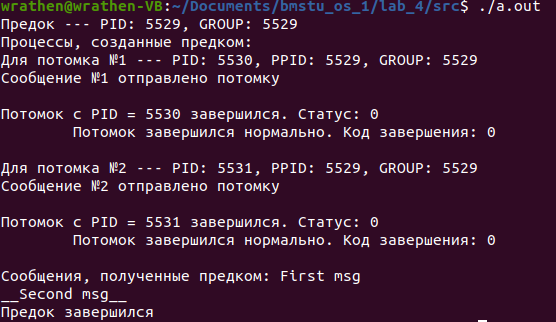
\includegraphics[width=\linewidth]{img/task_04.png}
		\caption{Демонстрация работы программы (задание №4).}
		
		\label{fig:task_04}
		
	\end{figure}

	\section*{Задание 5.}
	Предок и потомки аналогично №4 обмениваются сообщениями через неименованный программный канал.
	В программу включается собственный обработчик сигнала.
	С помощью сигнала меняется ход выполнения программы.
	При получении сигнала потомки записывают сообщения в канал, если сигнал не поступает, то не записывают.
	Предок ждет завершения своих потомков и анализирует коды их завершений.
	Вывод соответствующих сообщений на экран.
	
	\begin{lstlisting}[label=code:signal, caption=signal(), language=C]
		#include <stdio.h>
		#include <stdlib.h>
		#include <wait.h>
		#include <string.h>
		#include <signal.h>
		
		enum error_t {
			no_error,
			fork_fail,
			exec_fail,
			pipe_fail
		};
		
		#define PROC_COUNT 3
		#define SLEEP_TIME 2
		#define STR_BUFF_SIZE 64
		
		void do_nothing(int sigint) {
			printf("Ничего не происходит?\n");
		}
		
		static int sig_status = 0;
		
		void inc_status(int sigint) {
			sig_status++;
			printf("Статус увеличен - %d\n", sig_status);
		}
		
		int main() {
			int pipefd[2];  // [0] - чтение, [1] - запись
			if (pipe(pipefd) == -1) {
				perror("Ошибка pipe\n");
				return pipe_fail;
			}
			
			char *msgs[PROC_COUNT] = {"First msg\n", "Second msg\n", "Third message\n"};
			char str_buff[STR_BUFF_SIZE] = {0};
			
			int children[PROC_COUNT];
			printf("Предок --- PID: %d, GROUP: %d\n", getpid(), getpgrp());
			signal(SIGINT, do_nothing);
			
			for (int i = 0; i < PROC_COUNT; ++i) {
				int child_pid = fork();
				
				if (child_pid == -1) {
					perror("Ошибка fork'а");
					return fork_fail;
				}
				else if (child_pid == 0) {
					printf("Для потомка No%d --- PID: %d, PPID: %d, GROUP: %d\n", i + 1, getpid(), getppid(), getpgrp());
					
					signal(SIGINT, inc_status);
					sleep(SLEEP_TIME);
					
					if (sig_status != 0) {
						close(pipefd[0]);
						write(pipefd[1], msgs[i], strlen(msgs[i]));
						printf("Сообщение No%d отправлено потомку\n\n", i + 1);
					}
					else {
						printf("Сигнала не было\n\n");
					}
					
					return no_error;
				}
				else {
					children[i] = child_pid;
				}
			}
			
			printf("Процессы, созданные предком:\n");
			for (int i = 0; i < PROC_COUNT; ++i) {
				int status;
				int stat_value = 0;
				
				pid_t child_pid = wait(&status);
				printf("Потомок с PID = %d завершился. Статус: %d\n", children[i], status);
				
				if (WIFEXITED(stat_value)) {
					printf("\tПотомок завершился нормально. Код завершения: %d\n\n", WEXITSTATUS(stat_value));
				}
				else if (WIFSIGNALED(stat_value)) {
					printf("\tПотомок завершился неперехватываемым сигналом. Номер сигнала: %d\n\n", WTERMSIG(stat_value));
				}
				else if (WIFSTOPPED(stat_value)) {
					printf("\tПотомок остановился. Номер сигнала: %d\n\n", WSTOPSIG(stat_value));
				}
			}
			
			close(pipefd[1]);
			read(pipefd[0], str_buff, STR_BUFF_SIZE);
			printf("Сообщения, полученные предком: %s", str_buff);
			
			printf("Предок завершился\n");
			return no_error;
		}
	\end{lstlisting}

	\begin{figure}[H]
		
		\centering
		
		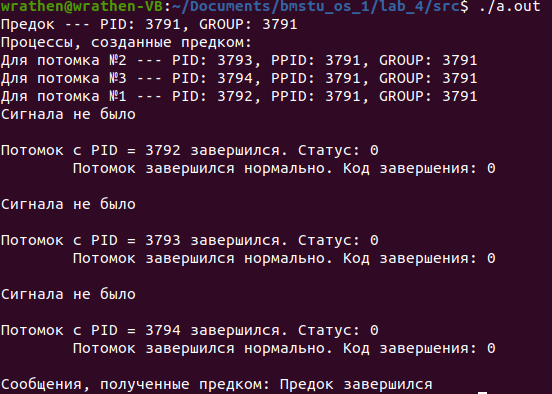
\includegraphics[width=\linewidth]{img/task_05.png}
		\caption{Демонстрация работы программы (задание №5).}
		
		\label{fig:task_05}
		
	\end{figure}
\end{document}